\documentclass[11pt,a4paper]{article}

\usepackage{fontspec}
\setmainfont{Arial}
\setsansfont{Arial}
\usepackage{polyglossia}
\setmainlanguage{russian}
\setotherlanguage{english}
\newfontfamily\cyrillicfont{Arial}
\newfontfamily\cyrillicfontsf{Arial}
\newfontfamily\cyrillicfonttt{Arial}
\usepackage{amsmath,amssymb}
\usepackage{geometry}
\usepackage{graphicx}
\usepackage{booktabs}
\usepackage{array}
\usepackage{tabularx}
\usepackage{longtable}
\usepackage{caption}
\usepackage{subcaption}
\usepackage{xcolor}
\usepackage{hyperref}
\usepackage[numbers,sort&compress]{natbib}
\usepackage{microtype}

\geometry{margin=24mm}
\hypersetup{
  colorlinks=true,
  linkcolor=blue!55!black,
  citecolor=blue!55!black,
  urlcolor=blue!55!black
}
\setlength{\parskip}{0.55em}
\setlength{\parindent}{0pt}
\sloppy

\newcommand{\R}{\mathbb{R}}
\newcommand{\Y}{\mathcal{Y}}
\newcommand{\X}{\mathcal{X}}
\newcommand{\argmax}{\operatorname*{arg\,max}}
\newcommand{\argmin}{\operatorname*{arg\,min}}
\newcommand{\norm}[1]{\left\lVert #1 \right\rVert}

\title{\textbf{Structural SVM OCR: математическая постановка и честное сравнение DBCFW vs DFW}}
\author{Эксперименты Decentralized Block-Coordinate Frank-Wolfe}
\date{22 июня 2026}

\begin{document}
\maketitle

\begin{abstract}
В этом документе описан эксперимент Structural SVM OCR из репозитория. Мы формализуем задачу предсказания последовательности, loss-augmented Viterbi oracle, primal- и dual-постановки Structural SVM, а также семейство методов Frank-Wolfe. Главный эмпирический результат не сравнивает центральный FW с децентрализованным DFW. Основное честное сравнение - это decentralized DBCFW против decentralized DFW на одном OCR split, с одной сетевой постановкой, одним регуляризатором и общей осью стоимости: числом обучающих loss-augmented Viterbi oracle calls. При таком учете DBCFW с одним блоком на агента достигает 18.24\% OCR test error за 3,780 training oracle calls, тогда как ближайшая точка DFW использует 6,251 calls и дает 72.20\% test error. Центральный BCFW приводится только как sanity reference и достигает 10.95\% best test error.
\end{abstract}

\section{Задача и данные}

Мы рассматриваем sequence labeling для датасета Taskar OCR, который часто используется в литературе по max-margin structured prediction \citep{taskar2003maxmargin,lacostejulien2013bcfw}. Каждый пример - это изображение слова, уже разбитое на символы. Вход представляет собой последовательность
\[
  x_i = (x_{i1},\ldots,x_{iT_i}), \qquad x_{it}\in\R^{129},
\]
где 128 пиксельных признаков дополнены постоянной bias-координатой. Выход - последовательность меток
\[
  y_i = (y_{i1},\ldots,y_{iT_i}), \qquad y_{it}\in\{1,\ldots,26\}.
\]
Мы используем split \texttt{ocr2}: folds, не равные нулю, идут в train, fold 0 идет в test. В локальном запуске это дает 6,251 обучающее слово и 626 тестовых слов. Общее число train letters равно 47,535, test letters - 4,617.

Структурная feature map раскладывается на emission-, boundary- и transition-признаки:
\[
  \Phi(x,y) =
  \left[
    \sum_{t=1}^{T} x_t \otimes e_{y_t},
    e_{y_1},
    e_{y_T},
    \sum_{t=2}^{T} e_{y_{t-1}}\otimes e_{y_t}
  \right].
\]
При 129 входных признаках, 26 метках, двух boundary-блоках и таблице переходов \(26\times26\) размерность равна
\[
  d = 129\cdot 26 + 2\cdot 26 + 26^2 = 4082.
\]
Предсказание задается как
\[
  h_w(x) = \argmax_{y\in\Y(x)} \langle w,\Phi(x,y)\rangle .
\]
Качество измеряется normalized Hamming loss:
\[
  \Delta(y,\hat y) = \frac{1}{T}\sum_{t=1}^{T}\mathbf{1}\{y_t\neq \hat y_t\}.
\]

\section{Постановка Structural SVM}

Мы используем margin-rescaled Structural SVM \citep{tsochantaridis2005large,joachims2009cutting}. Для каждого примера определим difference feature vector
\[
  \psi_i(y) = \Phi(x_i,y_i)-\Phi(x_i,y).
\]
Структурный hinge loss для примера \(i\):
\[
  H_i(w) = \max_{y\in\Y(x_i)}
    \left\{
      \Delta(y_i,y) - \langle w,\psi_i(y)\rangle
    \right\}.
\]
Primal objective:
\[
  P(w) =
  \frac{\lambda}{2}\norm{w}^2 +
  \frac{1}{n}\sum_{i=1}^{n} H_i(w).
\]
Loss-augmented inference problem:
\[
  \hat y_i(w) =
  \argmax_{y\in\Y(x_i)}
    \left\{
      \Delta(y_i,y) + \langle w,\Phi(x_i,y)\rangle
    \right\}.
\]
Для sequence model с переходами первого порядка эта задача точно решается динамическим программированием Viterbi. В нашем эксперименте один такой loss-augmented Viterbi call является дорогим атомарным oracle.

Dual-постановка, используемая Frank-Wolfe, имеет один simplex block на каждый обучающий пример:
\[
  \alpha_i \in \Delta_{\Y_i}, \qquad i=1,\ldots,n.
\]
Пусть
\[
  w(\alpha) =
  \frac{1}{\lambda n}
  \sum_{i=1}^{n}\sum_{y\in\Y_i}\alpha_i(y)\psi_i(y),
  \qquad
  \ell(\alpha) =
  \frac{1}{n}
  \sum_{i=1}^{n}\sum_{y\in\Y_i}\alpha_i(y)\Delta(y_i,y).
\]
Тогда concave dual objective:
\[
  D(\alpha) =
  \ell(\alpha) -
  \frac{\lambda}{2}\norm{w(\alpha)}^2.
\]
Frank-Wolfe duality gap можно вычислять через те же loss-augmented inference oracles. Это одна из причин, почему BCFW особенно естественен для Structural SVM \citep{lacostejulien2013bcfw}.

\section{Классические подходы}

\paragraph{Cutting-plane Structural SVM.}
Классическое обучение Structural SVM решает квадратичную программу с экспоненциальным числом margin constraints, итеративно добавляя violated constraints \citep{tsochantaridis2005large,joachims2009cutting}. Метод силен как batch-подход, но каждая крупная итерация требует inference по многим или всем примерам.

\paragraph{Full Frank-Wolfe.}
Классический Frank-Wolfe, или conditional gradient method \citep{frank1956algorithm,jaggi2013frankwolfe}, не требует проекций и использует linear minimization oracle. Для dual Structural SVM полный FW step запускает loss-augmented inference для всех train blocks, строит полный search vertex и затем делает convex update.

\paragraph{Block-coordinate Frank-Wolfe.}
BCFW обновляет один example block или mini-batch blocks за итерацию. Lacoste-Julien et al. показывают, что это хорошо подходит для Structural SVM: dual feasible set является декартовым произведением симплексов, а block oracle - это просто один loss-augmented inference problem \citep{lacostejulien2013bcfw}. Поэтому стоимость одной итерации резко ниже, чем у полного FW.

\paragraph{Decentralized Frank-Wolfe.}
Децентрализованные FW-методы совмещают conditional-gradient шаги с network averaging или consensus между агентами \citep{wai2017decentralized}. Наш эксперимент следует этой projection-free decentralized логике: агенты владеют разными частями OCR train set и обмениваются информацией через Erdos-Renyi graph.

\section{Что именно сравниваем}

Главное сравнение - decentralized DBCFW против decentralized DFW на одной задаче OCR Structural SVM. Важно не смешивать две разные пары сравнений:

\begin{enumerate}
  \item \textbf{Decentralized DBCFW vs DFW.} Это главный результат. Оба метода используют один train/test split, один regularization \(\lambda=1/n\), одно 7-agent разбиение, один graph seed и одну decentralized communication model. Методы различаются block budget: DBCFW использует \(B=1\), DFW использует полный локальный budget \(B=893\).
  \item \textbf{Central BCFW vs FW.} Это sanity/reference validation реализации Structural SVM в paper-style central setup. Это не baseline для DFW.
\end{enumerate}

Ось стоимости - \emph{training oracle calls}. Один training oracle call - это один loss-augmented Viterbi call, потраченный update-шагом. Диагностические вызовы, которые нужны только для test error или full duality gap, в эту ось не включаются.

Для decentralized OCR run:
\[
  \text{cost per DBCFW iteration with }B=1 = 7\cdot 1 = 7,
\]
тогда как
\[
  \text{cost per DFW iteration with }B=893 = 7\cdot 893 = 6251.
\]
Поэтому сравнение по raw iteration count было бы некорректным. DBCFW успевает сделать много дешевых block updates до того, как DFW завершит один полный локальный update. Честный вопрос: при сопоставимом числе loss-augmented Viterbi oracle calls какой метод дает меньший test error?

\section{Экспериментальный сетап}

Локальные артефакты, использованные в этом отчете:
\begin{itemize}
  \item \path{runs_paper_ocr/ocr_decentralized_fair_oracle_extra/results.csv}: основной fair sweep DBCFW vs DFW.
  \item \path{runs_paper_ocr/ocr_full_140_passes/results.csv}: central BCFW/FW sanity reference.
\end{itemize}
В decentralized fair sweep использовались:
\[
  N=7,\quad K=893,\quad \lambda\in\{0.01,0.001,1/n\}.
\]
Для DFW мы использовали полный block \(B=893\) и плотно логировали первые 25 итераций. Для DBCFW запускали \(B=1\) на 900 итераций, \(B=10\) на 200 итераций и \(B=89\) на 160 итераций.

\section{Главный результат}

\begin{figure}[htbp]
  \centering
  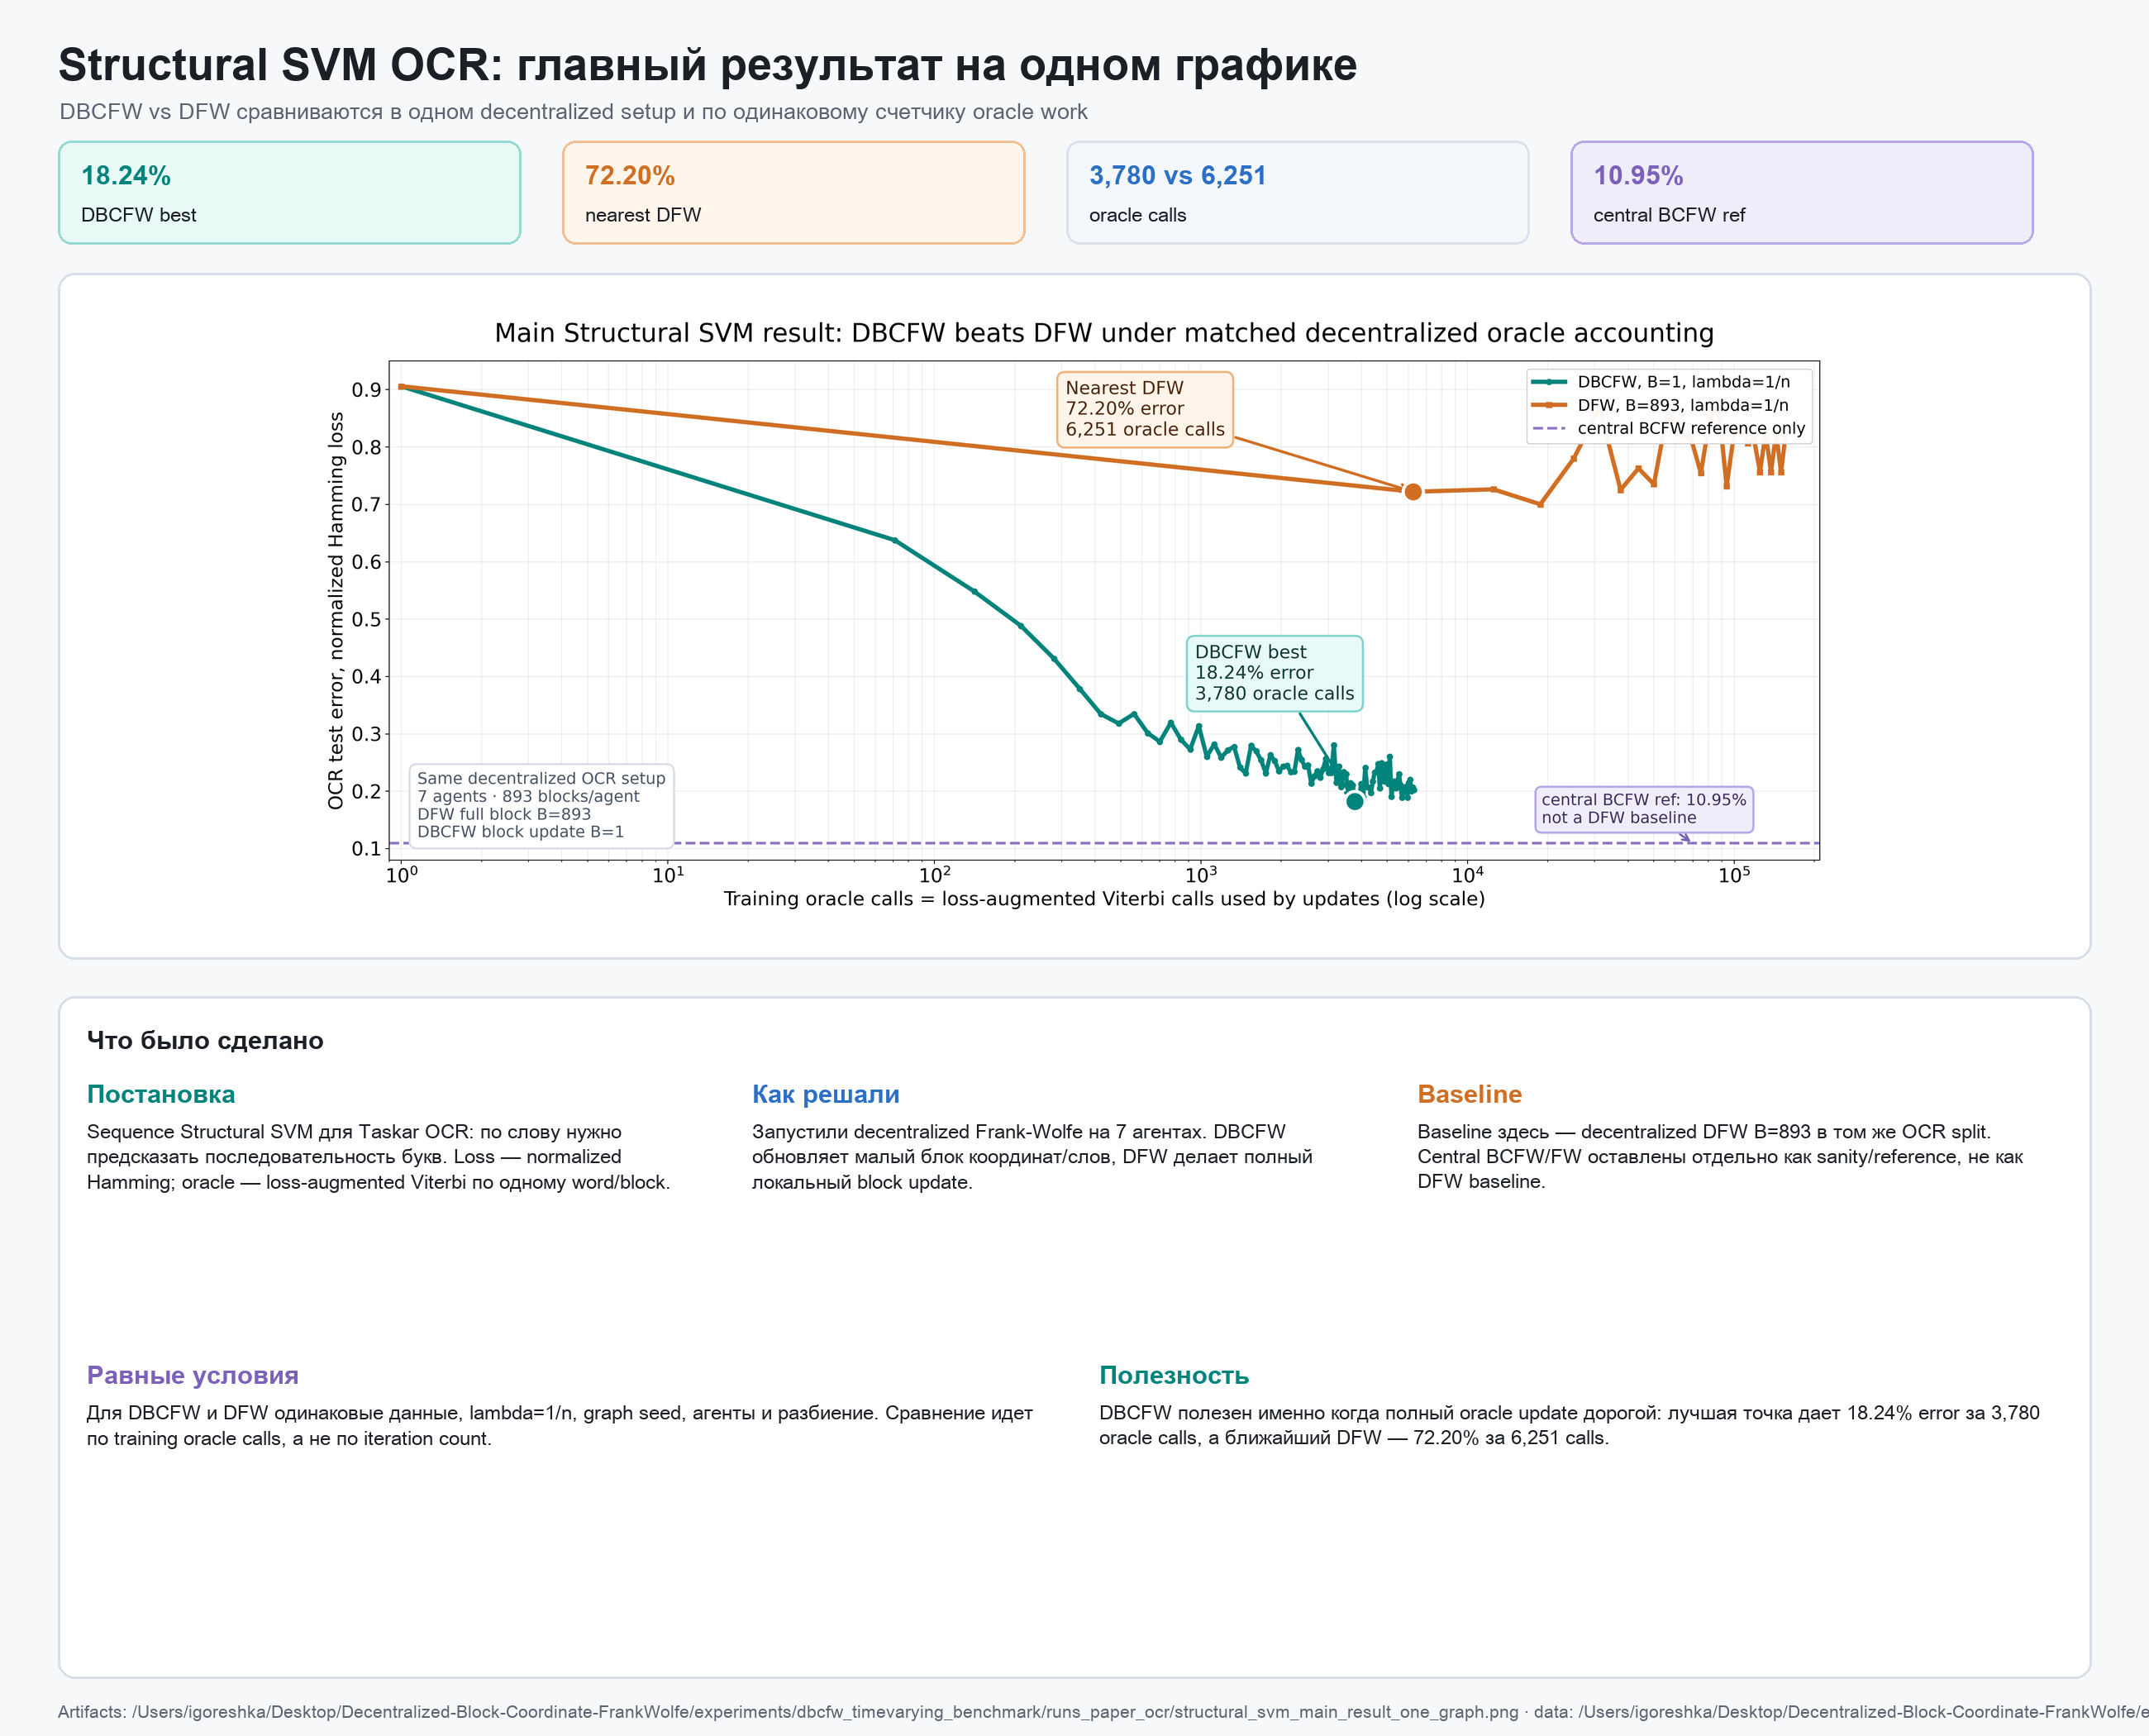
\includegraphics[width=\linewidth]{figures/main_result_one_graph.png}
  \caption{Главное fair-сравнение на Structural SVM OCR. DBCFW и DFW сравниваются в одном decentralized setup по training oracle calls на оси \(x\). Central BCFW показан только как reference line.}
  \label{fig:main-result}
\end{figure}

Лучшая fair-точка DBCFW в основном запуске:
\[
  \lambda = 1/n,\quad B=1,\quad \text{iteration}=540,\quad
  \text{training oracle calls}=3780.
\]
В этой точке test error равен \(18.24\%\). Ближайшая точка DFW для того же \(\lambda\) имеет 6,251 training oracle calls и \(72.20\%\) test error. Поэтому при oracle-work accounting DBCFW имеет примерно
\[
  \frac{72.20}{18.24}\approx 3.96
\]
раза меньший test error в выделенной точке сравнения.

\begin{table}[htbp]
\centering
\caption{Decentralized DBCFW vs DFW, matching по ближайшему training-oracle budget. Чем ниже test error, тем лучше.}
\resizebox{\linewidth}{!}{%
\begin{tabular}{llrrrrrrrrr}
\toprule
\(\lambda\) & \(B\) & DBCFW iter & DBCFW oracle & DBCFW test & DBCFW gap & DFW iter & DFW oracle & DFW test & DFW gap & ratio \\
\midrule
0.01  & 1  & 740 & 5180  & 19.11\% & 0.556 & 1  & 6251  & 72.20\% & 2      & 3.78x \\
0.01  & 10 & 55  & 3850  & 27.81\% & 8.31  & 1  & 6251  & 72.20\% & 2      & 2.60x \\
0.01  & 89 & 95  & 59185 & 58.92\% & 371   & 9  & 56259 & 84.99\% & 263    & 1.44x \\
0.001 & 1  & 580 & 4060  & 18.44\% & 0.568 & 1  & 6251  & 72.20\% & 2      & 3.91x \\
0.001 & 10 & 120 & 8400  & 28.31\% & 88.7  & 1  & 6251  & 72.20\% & 2      & 2.55x \\
0.001 & 89 & 155 & 96565 & 56.03\% & \(4.65{\times}10^3\) & 15 & 93765 & 68.21\% & \(2.63{\times}10^4\) & 1.22x \\
1/n   & 1  & 540 & 3780  & 18.24\% & 0.583 & 1  & 6251  & 72.20\% & 2      & 3.96x \\
1/n   & 10 & 75  & 5250  & 26.65\% & 546   & 1  & 6251  & 72.20\% & 2      & 2.71x \\
1/n   & 89 & 50  & 31150 & 56.86\% & \(3.62{\times}10^4\) & 5 & 31255 & 86.77\% & 30.8 & 1.53x \\
\bottomrule
\end{tabular}}
\label{tab:decentralized}
\end{table}

\section{Центральный sanity reference}

Central validation воспроизводит ожидаемое качественное поведение из литературы по BCFW для Structural SVM: BCFW существенно сильнее full central FW на этой OCR-задаче. Это подтверждает, что локальная постановка Structural SVM и loss-augmented Viterbi oracle работают разумно. Но это не baseline для decentralized DFW comparison.

\begin{table}[htbp]
\centering
\caption{Central BCFW vs FW validation. Таблица является sanity reference, а не decentralized DFW baseline.}
\begin{tabular}{lrrrrrrr}
\toprule
\(\lambda\) & BCFW best & pass & BCFW final gap & FW best & pass & FW final gap & ratio \\
\midrule
0.01  & 11.72\% & 20 & 0.00404 & 17.38\% & 137 & 0.627 & 1.48x \\
0.001 & 11.09\% & 35 & 0.0684  & 16.97\% & 138 & 0.692 & 1.53x \\
1/n   & 10.95\% & 75 & 0.221   & 17.72\% & 132 & 0.627 & 1.62x \\
\bottomrule
\end{tabular}
\label{tab:central}
\end{table}

\section{Почему сравнение справедливое}

Сравнение справедливо в следующем ограниченном смысле:
\begin{itemize}
  \item DBCFW и DFW используют один OCR split и одни train/test examples.
  \item Оба метода используют одно decentralized partition: 7 agents и 893 word blocks на агента.
  \item Оба используют одну graph model, seed и regularization value в выделенном результате.
  \item Оба измеряются по training loss-augmented Viterbi oracle calls - доминирующей дорогой операции в Structural SVM training.
  \item DFW baseline - это decentralized DFW, а не central FW.
\end{itemize}

Это не утверждение, что DBCFW универсально лучше при любой модели стоимости. DBCFW использует намного больше communication rounds: выделенная точка DBCFW использует 540 decentralized iterations, а ближайшая DFW точка - один full-block iteration. Поэтому сильнейшее утверждение, которое поддерживает эксперимент, - oracle efficiency: DBCFW существенно лучше, когда loss-augmented inference дорог относительно коммуникации.

\section{Почему DBCFW выигрывает здесь}

Главная причина - несоответствие гранулярности update и стоимости oracle. Один DFW step является полным локальным block update и стоит 6,251 loss-augmented Viterbi oracle calls. В том же oracle budget DBCFW с \(B=1\) может сделать сотни маленьких targeted block updates. В этом OCR run DBCFW получает полезную модель до того, как DFW успевает завершить даже один полный дорогой update.

Вторая причина - численная стабильность текущей decentralized реализации. В логах для \(\lambda=1/n\) выделенная точка DBCFW имеет test error \(18.24\%\), objective gap \(0.583\) и consensus error \(0.283\). DFW на более поздних итерациях развивает очень большие objective gaps и consensus errors. Это указывает, что full-block decentralized updates требуют более аккуратного scaling, line-search или state averaging, прежде чем они станут конкурентным baseline для этой Structural SVM-задачи.

\section{Вывод}

Эксперимент поддерживает следующий вывод:

\begin{quote}
Для decentralized Structural SVM OCR training block-coordinate decentralized Frank-Wolfe существенно более oracle-efficient, чем full-block decentralized Frank-Wolfe. Лучшая точка DBCFW достигает \(18.24\%\) test error за 3,780 training oracle calls, тогда как ближайшая точка DFW дает только \(72.20\%\) test error за 6,251 calls. Central BCFW остается лучше с \(10.95\%\), поэтому decentralized метод полезен, но пока не достигает central paper-quality performance.
\end{quote}

\bibliographystyle{plainnat}
\bibliography{references}

\end{document}
